\documentclass{fithesis}

\usepackage{lmodern}
\usepackage[czech]{babel}
\usepackage[utf8]{inputenc}
\usepackage{cmap}
\usepackage{graphicx}
\usepackage[T1]{fontenc} %formátuje české znaky - důležité
\usepackage[plainpages=false, pdfpagelabels]{hyperref}
\usepackage{hyperref}
%\usepackage{makeidx}
%\makeindex

%\bibliographystyle{unsrt}


%\makeindex
\thesistitle{Integrace DMS a workflow v Liferay Portal}
\thesissubtitle{Diplomová práce}
\thesisstudent{Marek Tlačbaba}
\thesiswoman{false}
\thesisfaculty{fi}
\thesisyear{2014}
\thesisadvisor{RNDr. Jaroslav Ráček, Ph.D.}


\begin{document}

\FrontMatter
\ThesisTitlePage

\begin{ThesisDeclaration}
Prohlášení\AdvisorName
\end{ThesisDeclaration}

\begin{ThesisThanks}
Poděkování
\end{ThesisThanks}

\begin{ThesisAbstract}
Abstrak
\end{ThesisAbstract}

\begin{ThesisKeyWords}
Klíčová slova
\end{ThesisKeyWords}


\MainMatter
\setcounter{secnumdepth}{4}
\tableofcontents

\chapter{Úvod}
Oficiální zadání

Popsat principy tvorby podnikových portálů. Zaměřit se zejména na otázku implementace workflow pro procesy pracující s vnitropodnikovými dokomenty. Pro Liferay Portal verze CE analyzovat, navrhnout, implementovat, otestovat a zdokumentovat vlastní grafický workflow editor pracující v základní notaci BPMN, který bude plně kompatibilní se standardním workflow systémem, který je součástí Liferay Potral CE. Výstup bude mít podobu funkčního prototypu.

\chapter{Podnikové portály}

Pojem portál bývá definován různými způsoby v závislosti na situaci, ve které je používán. Dříve se portály zaměřovaly hlavně a jenom kolem jednotného přístupu k informacím nezávisle na jejich původu a umístění. S~dalším vývojem informačních technologií se postupně tento přístup dále rozšiřoval a~do definice portálu přibyly pojmy jako integrace a agregace služeb a aplikací. 

V následujícím textu je uvedno několik definic portálu a podnikového portálu.

\begin{itemize}

\item Například Gála definoval portál jako jednotné rohraní, ve kterém lze pracovat s běžnými službami a nástroji jako jsou, například zpravodajství a~komunikace, mimo to je v něm zaručen přístup k všeobecným aplikacím jako jsou vlastní stránky a blogy, a k aplikacím specializovaným, například slovníkům. \cite{gala}

\item Tato definice portálu je převzata ze standardu JSR-286 a zní následovně: Portál je webová aplikace, která (obvykle) poskytuje možnost personalizace, autentifikace, agregace obsahu z různých zdrojů a slouží jako prezentační vrstva informačních systémů. Agregací se rozumí integrace obsahu z různých zdrojů v rámci jedné webové stránky. Portál může mít vysoce propracované nástroje pro personalizaci, které poskytují obsah upravitelný podle přání uživatele. Stránky portálu mohou mít různé skupiny portletů \footnote[1]{odkaz na portlet}, které vytvářejí obsah pro různé uživatele.  \cite{jsr-286}

\item Předchozí defince se týkají portálu obecně, proto zde uvedu také definici podnikového portálu jako takového. Například podle Čecha je podnikový portál definován jako internetové nebo intranetové stránky, které slouží jako vstupní bod, respektive brána k různým datovým, informačním a znalostním zdrojům v organizaci. Jejich cílem je zpřístupnit tyto zdroje specifické skupině lidí. Může to být jak zákazníkům, tak také vlastním zaměstnacům nebo partnerům. \cite{cech}

\end{itemize}

V předchozích definicích portálu jsou naznačeny některé základní rysy podnikových portálů. Mezi základní vlastnosti můžeme považovat jediný přístupový bod, integrace, federace, přizpůsobivost, personalizace, kontrola přístupu a vyhledávání v podnikovém obsahu, tak jak jsou uvedeny v \cite{enterprise-portal} 




\chapter{Vzorová kapitola}
\section{Vzorová sekce}
\subsection{Vzorová podsekce}

\begin{figure}[htp]
\centering
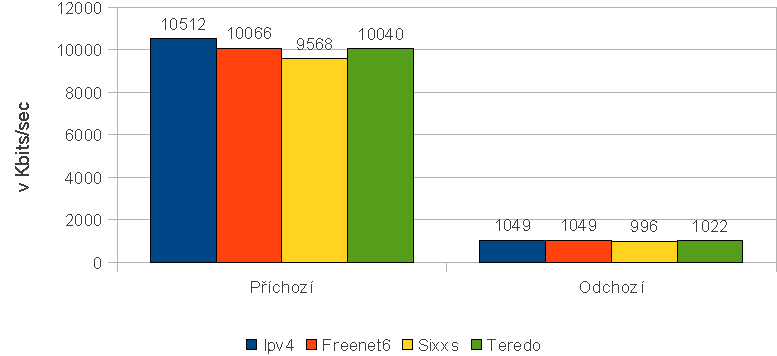
\includegraphics[width=340px]{images/bandwith.pdf}
\caption{Vzorový obrázek}
\end{figure}

\begin{itemize}
\item vzorový seznam
\end{itemize}


\begin{table}
\centering
\begin{tabular}{|p{3cm}|p{8cm}|}
\hline Sloupec 1 & Sloupec 2 \\
\hline Položka 2 & položka 2 \\
\hline
\end{tabular}
\caption{Vybrané skupinové adresy (převzato z \cite{satrapa-ipv6})}
\end{table}



%\printindex

\begin{thebibliography}{0}

\bibitem{gala}
GÁLA, L. et al. \textit{Podniková informatika}. 1. vyd. Praha: Grada Publishing, 2006. 

\bibitem{jsr-286}
\textit{JavaTM Portlet Specification}, The Java Community Process, dostupný na \url{http://www.jcp.org/en/jsr/detail?id=286} [cit. 2014-03-27].

\bibitem{cech}
ČECH, P. \textit {Přinos podnikových portálů pro management znalostí}, in Internet a konkurenceschopnost, Zlín, 2004.

\bibitem{enterprise-portal}
\textit{Enterprise portal}, Wikipedia, dostupný na \url{http://en.wikipedia.org/wiki/Enterprise_portal} [cit. 2014-03-27].






\end{thebibliography}


\newpage
\appendix
\chapter{Položky seznamu}
asdfsadf

\chapter{Položky seznamu}
asdfsadf


\end{document}